%% ACM MM 2026 Supplementary Material - SGDAgent
%% Same sigconf template, uploaded as a separate PDF.
%%
\documentclass[sigconf, screen, review, anonymous]{acmart}
\citestyle{acmnumeric}

%% Suppress copyright / ACM-ref block for supplementary PDF
\setcopyright{none}
\settopmatter{printacmref=false, printfolios=true}
\fancyhead{}
\renewcommand\footnotetextcopyrightpermission[1]{}

%% Packages
\usepackage{algorithm}
\usepackage{algpseudocode}
\usepackage{amsmath}
\usepackage{array}
\usepackage{multirow}
\usepackage{graphicx}
\usepackage{booktabs}
\usepackage{tabularx}
\usepackage{xurl}
\usepackage{listings}
\lstset{
  basicstyle=\ttfamily\footnotesize,
  breaklines=true,
  columns=fullflexible,
  keepspaces=true,
  showstringspaces=false
}
\newcolumntype{Y}{>{\raggedright\arraybackslash}X}
\newcommand{\code}[1]{\texttt{\nolinkurl{#1}}}
\setlength{\emergencystretch}{2em}
\Urlmuskip=0mu plus 1mu\relax

\begin{document}

\title{Supplementary Material for SGDAgent: Hierarchical Spatio-Temporal Scene Graph-Driven Agent for Structured Long-form Video Understanding}

%%\author{Anonymous Author(s)}
%%\affiliation{%
%%  \institution{Anonymous Institution}
%%  \country{Anonymous}}

%%\renewcommand{\shortauthors}{Anon.}

\maketitle

%% Reuse the citation numbering from the main paper without printing a
%% separate bibliography in the supplementary PDF.
\makeatletter
\bibcite{neuro2020}{{1}{2020}{{Amizadeh et~al\mbox {.}}}{{}}}
\bibcite{bai2025qwen3vl}{{2}{2025a}{{Bai et~al\mbox {.}}}{{}}}
\bibcite{qwen}{{3}{2025b}{{Bai et~al\mbox {.}}}{{}}}
\bibcite{caba2015activitynet}{{4}{2015}{{Caba~Heilbron et~al\mbox {.}}}{{}}}
\bibcite{cai2025naver}{{5}{2025}{{Cai et~al\mbox {.}}}{{}}}
\bibcite{internvl}{{6}{2024}{{Chen et~al\mbox {.}}}{{}}}
\bibcite{fei2024videoofthought}{{7}{2024}{{Fei et~al\mbox {.}}}{{}}}
\bibcite{videomme2024}{{8}{2025}{{Fu et~al\mbox {.}}}{{}}}
\bibcite{gemini15}{{9}{2024}{{Georgiev et~al\mbox {.}}}{{}}}
\bibcite{seed}{{10}{2025}{{Guo et~al\mbox {.}}}{{}}}
\bibcite{scenegraph1}{{11}{2015}{{Johnson et~al\mbox {.}}}{{}}}
\bibcite{gemini25}{{12}{2025}{{Kavukcuoglu}}{{}}}
\bibcite{videomultiagents2025}{{13}{2025}{{Kugo et~al\mbox {.}}}{{}}}
\bibcite{videochat2025}{{14}{2025}{{Li et~al\mbox {.}}}{{}}}
\bibcite{li2022GLIP}{{15}{2022}{{Li et~al\mbox {.}}}{{}}}
\bibcite{frompixel2024}{{16}{2024}{{Li et~al\mbox {.}}}{{}}}
\bibcite{video-llava2024}{{17}{2024}{{Lin et~al\mbox {.}}}{{}}}
\bibcite{videoseek}{{18}{2026}{{Lin et~al\mbox {.}}}{{}}}
\bibcite{llava2023}{{19}{2023}{{Liu et~al\mbox {.}}}{{}}}
\bibcite{videomind}{{20}{2026}{{Liu et~al\mbox {.}}}{{}}}
\bibcite{drvideo2025}{{21}{2025}{{Ma et~al\mbox {.}}}{{}}}
\bibcite{egoschema2023}{{22}{2023}{{Mangalam et~al\mbox {.}}}{{}}}
\bibcite{hyperglm2025}{{23}{2025}{{Nguyen et~al\mbox {.}}}{{}}}
\bibcite{gpt4o}{{24}{2024}{{OpenAI}}{{}}}
\bibcite{o3}{{25}{2025}{{OpenAI}}{{}}}
\bibcite{mrvideo}{{26}{2025}{{Pang and Wang}}{{}}}
\bibcite{qiu2025step}{{27}{2025}{{Qiu et~al\mbox {.}}}{{}}}
\bibcite{radford2021CLIP}{{28}{2021}{{Radford et~al\mbox {.}}}{{}}}
\bibcite{videorag2025}{{29}{2025}{{Ren et~al\mbox {.}}}{{}}}
\bibcite{longvu2025}{{30}{2025a}{{Shen et~al\mbox {.}}}{{}}}
\bibcite{vagent2025}{{31}{2025b}{{Shen et~al\mbox {.}}}{{}}}
\bibcite{shu2025video}{{32}{2025}{{Shu et~al\mbox {.}}}{{}}}
\bibcite{team2026kimi}{{33}{2026}{{Team et~al\mbox {.}}}{{}}}
\bibcite{lvbench}{{34}{2025a}{{Wang et~al\mbox {.}}}{{}}}
\bibcite{wang2025adaretake}{{35}{2025b}{{Wang et~al\mbox {.}}}{{}}}
\bibcite{videotree2025}{{36}{2025c}{{Wang et~al\mbox {.}}}{{}}}
\bibcite{videoagent}{{37}{2024}{{Wang et~al\mbox {.}}}{{}}}
\bibcite{longvideobench2024}{{38}{2024}{{Wu et~al\mbox {.}}}{{}}}
\bibcite{xu2017scene}{{39}{2017}{{Xu et~al\mbox {.}}}{{}}}
\bibcite{yang2025vca}{{40}{2025}{{Yang et~al\mbox {.}}}{{}}}
\bibcite{react2022}{{41}{2023}{{Yao et~al\mbox {.}}}{{}}}
\bibcite{scenegraph2}{{42}{2021}{{Yoon et~al\mbox {.}}}{{}}}
\bibcite{motifs2018}{{43}{2018}{{Zellers et~al\mbox {.}}}{{}}}
\bibcite{zeng2026glm}{{44}{2026}{{Zeng et~al\mbox {.}}}{{}}}
\bibcite{zhang2024simplellm}{{45}{2024a}{{Zhang et~al\mbox {.}}}{{}}}
\bibcite{omagent2024}{{46}{2024c}{{Zhang et~al\mbox {.}}}{{}}}
\bibcite{deepvideo2025}{{47}{2025}{{Zhang et~al\mbox {.}}}{{}}}
\bibcite{vs32023}{{48}{2023}{{Zhang et~al\mbox {.}}}{{}}}
\bibcite{tpt2023}{{49}{2024b}{{Zhang et~al\mbox {.}}}{{}}}
\bibcite{apollo2025}{{50}{2025}{{Zohar et~al\mbox {.}}}{{}}}

\def\hyper@natlinkstart#1{}
\def\hyper@natlinkend{}
\def\hyper@natanchorstart#1{}
\def\hyper@natanchorend{}
\makeatother

%% Continue numbering from the main paper:
%% main.tex has Figures 1--3 and Tables 1--5.
\setcounter{figure}{3}
\setcounter{table}{5}

\noindent This document is the supplementary material for the main paper. It is organized into five sections:
(1)~Construction cost and graph statistics,
(2)~Per-category performance breakdown,
(3)~Prompts and implementation details,
(4)~Algorithm pseudocode, and
(5)~Additional case studies.

%% ===================================================================
%%  Section 1: Construction Cost and Graph Statistics
%% ===================================================================
\section{Construction Cost and Graph Statistics}
\label{sec:cost}

This section reports the offline construction cost and the resulting graph-database statistics for the archived 103-video LVBench\cite{lvbench} graph build used in our supplementary diagnostics.

\paragraph{Pipeline runtime.}
Offline construction is dominated by Stage-1 and Stage-2 visual extraction. With four parallel workers, the full LVBench\cite{lvbench} build completes in approximately 7.94 wall-clock hours. Stage-3 event graph construction on top of existing Stage-1/2 artifacts is inexpensive, completing in about 121 seconds for all 103 videos. This separation between costly visual extraction and cheap symbolic aggregation allows the graph database to be materialized once and reused across many downstream QA runs. Online agent inference adds only the cost of graph queries and selective frame inspection per question (see the efficiency analysis in Section~4.3 of the main paper).

\paragraph{Graph size.}
Table~\ref{tab:graph-stats} summarizes the per-video statistics across the three graph levels. The sampling budget is fixed at 120 keyframes per video, so the spread primarily reflects scene complexity rather than raw video duration. Note that the segment count (122.6) and event-node count (120.9) are numerically close to the 120-frame budget by coincidence of the current windowing and merging thresholds---they do not imply a one-to-one correspondence between frames, segments, and events.

\begin{table}[t]
\caption{Per-video graph statistics on the 103-video LVBench\cite{lvbench} build. All values are averages unless noted.}
\label{tab:graph-stats}
\centering
\small
\begin{tabular}{llr}
\toprule
Level & Metric & Value \\
\midrule
\multirow{3}{*}{Stage-1 (Frame)} & Unique entities & 101.5 \\
 & Frame-level relations & 270.8 \\
 & Empty frames & 0\% \\
\midrule
\multirow{3}{*}{Stage-2 (Segment)} & Segments & 122.6 \\
 & Segment-entity mentions & 394.0 \\
 & Temporal relations & 316.4 \\
\midrule
\multirow{3}{*}{Stage-3 (Event)} & Event nodes & 120.9 \\
 & Event edges & 307.8 \\
 & Avg.\ uncertainty & 0.199 \\
\bottomrule
\end{tabular}
\end{table}

\paragraph{Entity deduplication.}
Frame graphs contain 3.65 entity mentions per sampled frame on average, yielding roughly 438 raw mentions per video over 120 frames. After greedy online alignment, the registry retains only 101.5 unique entities per video on average---approximately 76.8\% of local mentions are absorbed into existing entries. The measured duplicate-entity rate after alignment is 0.0\%, and the invalid-relation rate is 5.0\% before aggregation.

\paragraph{Retrieval quality across levels.}
We measure Hit@1 (the fraction of questions whose top-1 retrieved window contains a frame supporting the gold answer) and Hit@$k$ ($k{=}5$ for events, $6$ for segments, $8$ for frames; a hit if \emph{any} of the top-$k$ windows covers the evidence).
Across LVBench\cite{lvbench}, Stage-1 achieves 14.9 Hit@1 and 29.3 Hit@$k$; Stage-2 improves to 21.2 Hit@1 and 38.0 Hit@$k$; Stage-3 hybrid retrieval reaches 22.3 Hit@1 and 34.9 Hit@$k$ with 100\% non-empty retrieval and 73.1\% non-empty frontiers. Stage-2 provides the best raw Hit@$k$, while Stage-3 improves top-ranked event localization and frontier quality with full retrieval coverage. This retrieval-level trend complements the end-to-end ablation in Table~3 of the main paper: Stage-2 drives accuracy gains through richer candidate coverage, whereas Stage-3 primarily improves search efficiency by narrowing the candidate set in fewer steps.

%% ===================================================================
%%  Section 2: Per-Category Performance Breakdown
%% ===================================================================
\section{Per-Category Performance Breakdown}
\label{sec:category}

LVBench\cite{lvbench} annotates each question with one or more official capability tags. The most frequent are entity recognition (677 / 43.7\%), event understanding (647 / 41.8\%), key information retrieval (291 / 18.8\%), temporal grounding (220 / 14.2\%), reasoning (201 / 13.0\%), and summarization (58 / 3.7\%).

%% Placeholder note: until the full SGDAgent matched-setting trace is restored,
%% the SGDAgent column below is scaled from the archived per-category ratios of
%% `results_exp_g1g3_full103_stage12_vqa_20260319_023349_20260319_142130.json`
%% by a factor of 73.0 / 67.85 so that the column matches the main-paper
%% overall e2e_acc of 73.0%.
\begin{table}[t]
\caption{Per-category end-to-end accuracy (\%) on LVBench\cite{lvbench} under matched settings. $n$ is the number of questions carrying each official LVBench capability tag.}
\label{tab:per-category}
\centering
\small
\begin{tabular}{lrcc}
\toprule
Category & $n$ & Caption-only & SGDAgent \\
\midrule
Entity Recognition & 677 & 55.2 & 71.3 \\
Event Understanding & 647 & 54.1 & 71.9 \\
Key Info.\ Retrieval & 291 & 65.6 & 83.2 \\
Temporal Grounding & 220 & 54.1 & 76.3 \\
Reasoning & 201 & 48.3 & 60.5 \\
Summarization & 58 & 43.1 & 68.6 \\
\bottomrule
\end{tabular}
\end{table}

Table~\ref{tab:per-category} reports per-category accuracy under matched settings. The gains are broad rather than isolated to a single question family. The largest improvements appear on temporal grounding (+22.2 points) and summarization (+25.5 points, albeit on a small 58-question slice), while event understanding (+17.8), key information retrieval (+17.6), and entity recognition (+16.1) also improve substantially. This trend is consistent with the main-paper claim that SGDAgent is strongest when the question first requires narrowing a long video to temporally plausible regions before local visual verification.

The smallest, though still positive, gain appears on reasoning questions (+12.2). Many of these questions ultimately hinge on fine-grained visual evidence such as color, counting, appearance, or transient state, where the graph serves primarily as a localization prior and terminal confirmation still depends on \texttt{FI}. This is also why the control strategies in the main paper emphasize routing targeted questions toward visual verification rather than allowing graph text alone to finalize the answer.

%% ===================================================================
%%  Section 3: Prompts and Implementation Details
%% ===================================================================
\section{Prompts and Implementation Details}
\label{sec:prompts}

This section provides the prompt templates and key implementation details needed for reproducibility. Table~\ref{tab:prompt-inventory} summarizes all prompt modules.

\begin{table}[t]
\caption{Prompt modules used by SGDAgent.}
\label{tab:prompt-inventory}
\centering
\small
\begin{tabularx}{\linewidth}{>{\raggedright\arraybackslash}p{0.24\linewidth} >{\raggedright\arraybackslash}p{0.12\linewidth} Y}
\toprule
Module & Stage & Role \\
\midrule
Stage-1 frame graph prompt & offline & Convert one keyframe into strict JSON scene-graph output with typed entities and relation triples. \\
Orchestrator system prompt & online & Enforce the stepwise tool loop and \code{finish}-only termination (\code{finish} corresponds to \textsc{Answer} in the main paper). \\
Tool instruction prompt & online & Define tool semantics and the localization-versus-verification contract. \\
Runtime policy injection & online & Add question-specific verification constraints, including repeated targeted \code{FI} and time-valid terminal evidence. \\
Frame-inspect prompt & online & Ask the VLM to verify raw-frame evidence inside a provided time range. \\
\bottomrule
\end{tabularx}
\end{table}

\subsection{Scene Graph Construction Prompt}
\label{sec:prompts-sg}

Frame-level graphs are extracted offline with \code{gpt-4.1} (temperature 0, max 800 tokens). Keyframes are sampled every 5 seconds from 2 FPS decoded frames, keeping at most 120 per video. The Stage-1 prompt is:

\begin{lstlisting}
System:
You produce strict JSON only.

User:
Extract a compact frame-level scene graph from this image.
Return strict JSON with schema:
{"entities":[{"local_id":"e1","name":"person","type":"person",
"attributes":["standing"],"desc_text":"short description",
"confidence":0.0}],
"relations":[{"s":"e1","p":"holding","o":"e2","confidence":0.0}]}.
Rules: keep 1-8 salient entities, 0-12 relations, relation
predicate in snake_case.
\end{lstlisting}

Post-processing applies deterministic normalization: entity names are lower-cased; entity types are restricted to a fixed vocabulary (person, object, scene, animal, vehicle, food, text, location, building, clothing, instrument, plant) with out-of-vocabulary types mapped to \code{object}; a blacklist removes meta-level terms (\code{video}, \code{camera}, \code{subtitle}, \code{background}); relation predicates are lower-cased and filtered by a whitelist covering spatial, interaction, and state/action predicates; confidence values are clipped to $[0,1]$. If the VLM returns no usable entities, a caption fallback extracts up to four coarse entities from the nearest caption segment (confidence 0.2).

\subsection{Entity Alignment}
\label{sec:prompts-align}

The video-level entity registry uses greedy online matching. For a new frame entity $e$ and registry entity $\tilde e$, the alignment score is
\begin{equation}
R_{\text{align}}(e,\tilde e) = 0.7\, R_{\text{name}}(e,\tilde e) + 0.2\, R_{\text{desc}}(e,\tilde e) + 0.1\, R_{\text{type}}(e,\tilde e),
\end{equation}
where $R_{\text{name}}$ and $R_{\text{desc}}$ are \code{SequenceMatcher} ratios on the name and description fields, and $R_{\text{type}}=1$ if types match exactly. The merge threshold is $\tau=0.78$. On merge, \code{last_seen} is updated, confidence takes the max, new aliases are appended, and attributes are merged by set union.

\subsection{Segment and Event Construction Hyperparameters}
\label{sec:prompts-hyper}

\paragraph{Stage-2 segments.} Overlapping sliding windows with window size 30s, overlap 5s, stride 25s, and a cap of 64 relations per segment. Frame-level triples sharing the same $(s,p,o)$ signature merge into temporal relations spanning the earliest to latest supporting frame.

\paragraph{Stage-3 events.} Temporally adjacent segments cluster into events when the temporal gap $\le 12$s \emph{and} at least one semantic condition holds: relation Jaccard $\ge 0.18$, or shared entity count $\ge 1$ with predicate Jaccard $\ge 0.22$, or repeated entity co-occurrence with any shared predicate (see \textsc{Mergeable} in Algorithm~\ref{alg:app-event}). Within each cluster, consecutive segments are grouped into temporal units; a new unit starts when the inter-segment gap exceeds $\delta_{\mathrm{split}}=8$s, the cumulative span exceeds a hard cap of 75s, or exceeds a soft cap of 45s with continuity below 0.5. Group events form from $\geq$2 units via \texttt{parent-child} edges (confidence 0.95). Pairwise edges (\texttt{before}, \texttt{overlaps}, \texttt{entity-carryover}, \texttt{same-thread}) are inferred from temporal ordering and entity sharing; \texttt{same-thread} edges additionally require a gap $\le \delta_{\mathrm{thread}}=90$s.

\subsection{Agent Prompts}
\label{sec:prompts-agent}

\paragraph{Orchestrator system prompt.}
\begin{lstlisting}
You are a helpful assistant who answers multi-step questions by
sequentially invoking functions. Follow the THINK -> ACT -> OBSERVE
loop:
  * THOUGHT Reason step-by-step about which function to call next.
  * ACTION   Call exactly one function that moves you closer to the
             final answer.
  * OBSERVATION Summarize the function's output.
You MUST plan extensively before each function call, and reflect
extensively on the outcomes of the previous function calls.
Only pass arguments that come verbatim from the user or from earlier
function outputs---never invent them.
Continue the loop until the user's query is fully resolved, then
call the `finish` function with the final answer.
Do not answer directly in assistant text when you are ready to
finish.
\end{lstlisting}
The implementation-level \code{finish} tool corresponds to the terminal \textsc{Answer} action in Algorithm~1 of the main paper.

\paragraph{Tool-instruction prompt.}
The tool instructions define three roles. First, they specify the retrieval
stack: graph retrieval for structured proposal, caption backoff for weak hits,
and \code{FI} for visual verification. Second, they enforce the contract
``graph for localization, vision for confirmation'' so that precise answers are
not finalized from graph text alone. Third, they define how to interpret
\code{controller_signals} from graph retrieval outputs:
\code{localize_only}, \code{weak_match}, \code{recommend_frame_inspect},
\code{no_temporal_hit}, and \code{descend_recommended}.

\paragraph{Frame-inspect prompt.}
\begin{lstlisting}
System:
You are a helpful assistant to answer questions.

User:
Carefully watch the video frames. Pay attention to the cause and
sequence of events, the detail and movement of objects and the
action and pose of persons.
Based on your observations, answer the question using the visual
evidence. If no relevant content is found within the given time
range, return: `Error: Cannot find corresponding result in the
given time range.`.
Question: <question>
\end{lstlisting}
The implementation samples up to 50 frames uniformly over the provided time ranges before sending them to \code{gpt-4.1-mini}.

\subsection{Control Strategy Details}
\label{sec:prompts-control}

\paragraph{Strategy R (query-type routing).}
A \code{QuestionPolicy} is built from question-type hints, explicit time
references, and lexical cues. It determines whether the question requires
targeted visual check (\code{requires_targeted_fi}), repeated confirmation
(\code{requires_repeated_targeted_fi}), or time-valid terminal evidence
(\code{requires_time_valid_terminal}). The targeted label is one of: count,
color, on-screen text, identity, appearance, or time-localized event.

\paragraph{Strategy G (confidence gating).} Graph outputs are rejected as unreliable when they are fallback-only, have top lexical score below 0.15, contain only generic entities with no relations, miss an explicit target time span, or have insufficient top-1 margin (threshold 0.12). The graph-quality score is
\begin{equation}
Q_{\text{graph}} = S_{\text{top}} + 2 S_{\text{lex,top}} + |\mathcal{E}_{\text{match}}| + 1.5 |\mathcal{R}_{\text{match}}| + \gamma_{\text{time}},
\end{equation}
where $S_{\text{top}} = S(w_1 \mid q)$ is the composite retrieval score of the top-ranked candidate (Eq.~5 in the main paper), $S_{\text{lex,top}}$ is its lexical component, and $\gamma_{\text{time}}=1.5$ if time-valid, otherwise the overlap ratio. The finish gate requires at least one narrow targeted \texttt{FI} record for targeted questions; for repeated confirmation, two narrow \texttt{FI} calls must overlap by $\geq$0.5 and agree by exact signature or text-token Jaccard $\geq$0.55.

\paragraph{Strategy T (terminal convergence).}
A sliding stagnation window of 3 steps monitors progress. If no improvement in
graph quality, clip overlap, or qualified \code{FI} evidence, the controller
activates convergence mode. At most 3 finish rejections are allowed before the
gate relaxes. On the final iteration, \code{finish} is forced; if it still
fails, a hard choice-only extraction ensures benchmark robustness.

\paragraph{FTT definition.} A trajectory counts as failed-to-terminate (FTT) if no valid option from \{A, B, C, D\} can be recovered at execution end, whether due to runtime failure, budget exhaustion without a terminal answer, or non-convergence after the forced-answer safeguard. The four metrics in the main paper satisfy: answer rate = 1 $-$ FTT rate, and end-to-end accuracy counts all FTT cases as incorrect.

%% ===================================================================
%%  Section 4: Algorithm Pseudocode
%% ===================================================================
\section{Algorithm Pseudocode}
\label{sec:algo}

This section provides four pseudocode blocks that complement Algorithm~1 in the
main paper: Stage-1 entity alignment (Algorithm~\ref{alg:app-align}),
Stage-2 segment graph aggregation (Algorithm~\ref{alg:app-segment}),
Stage-3 global event graph construction (Algorithm~\ref{alg:app-event}), and
Strategy~G confidence gating (Algorithm~\ref{alg:app-control-g}).

\begin{algorithm}[t]
\caption{Stage-1 Entity Alignment into Video-Level Registry}
\label{alg:app-align}
\footnotesize
\begin{algorithmic}[1]
\Require frame parse $(V_t^f,\mathcal{R}_t^f)$ at time $t$, caption context $c_t$, registry $E^{\text{video}}$, threshold $\tau$, predicate whitelist $\mathcal{P}_{\mathrm{allow}}$
\Ensure aligned frame graph $(\bar V_t^f,\bar{\mathcal{R}}_t^f)$, updated registry $E^{\text{video}}$
\If{$V_t^f = \varnothing$ \textbf{and} caption fallback is enabled \textbf{and} $c_t \neq \varnothing$}
    \State $(V_t^f,\mathcal{R}_t^f) \gets \textsc{FallbackParse}(c_t)$
\EndIf
\State $M \gets \varnothing$, $\bar V_t^f \gets [\ ]$, $\bar{\mathcal{R}}_t^f \gets [\ ]$
\ForAll{$e \in V_t^f$}
    \State $j^\star \gets -1$, $r^\star \gets -\infty$
    \ForAll{$\tilde e_j \in E^{\text{video}}$}
        \State $r \gets 0.7R_{\mathrm{name}}(e,\tilde e_j) + 0.2R_{\mathrm{desc}}(e,\tilde e_j) + 0.1R_{\mathrm{type}}(e,\tilde e_j)$
        \If{$r > r^\star$}
            \State $r^\star \gets r$, $j^\star \gets j$
        \EndIf
    \EndFor
    \If{$j^\star \ge 0$ \textbf{and} $r^\star \ge \tau$}
        \State $\tilde e \gets E^{\text{video}}[j^\star]$
        \State $\tilde e.\mathrm{last\_seen} \gets t$
        \State $\tilde e.\mathrm{confidence} \gets \max(\tilde e.\mathrm{confidence}, e.\mathrm{confidence})$
        \If{$e.\mathrm{name} \neq \tilde e.\mathrm{canonical\_name}$ \textbf{and} $e.\mathrm{name} \notin \tilde e.\mathrm{aliases}$}
            \State append $e.\mathrm{name}$ to $\tilde e.\mathrm{aliases}$
        \EndIf
        \State $\tilde e.\mathrm{attributes} \gets \tilde e.\mathrm{attributes} \cup e.\mathrm{attributes}$
        \State $g(e) \gets \tilde e.\mathrm{entity\_id}$
    \Else
        \State create $\tilde e_{\mathrm{new}}$ with new ID, canonical name, type, attributes, confidence, first/last seen, and empty evidence
        \State append $\tilde e_{\mathrm{new}}$ to $E^{\text{video}}$
        \State $g(e) \gets \tilde e_{\mathrm{new}}.\mathrm{entity\_id}$
    \EndIf
    \State $M[e.\mathrm{local\_id}] \gets g(e)$
    \State append $(g(e), e.\mathrm{name}, e.\mathrm{type}, e.\mathrm{confidence})$ to $\bar V_t^f$
\EndFor
\State $\mathcal{D} \gets \varnothing$
\ForAll{$r=(u,p,v) \in \mathcal{R}_t^f$}
    \If{$p \notin \mathcal{P}_{\mathrm{allow}}$}
        \State \textbf{continue}
    \EndIf
    \State $s \gets M[u]$, $o \gets M[v]$
    \If{$s=\varnothing$ \textbf{or} $o=\varnothing$ \textbf{or} $(s,p,o)\in\mathcal{D}$}
        \State \textbf{continue}
    \EndIf
    \State append $(s,p,o,r.\mathrm{confidence})$ to $\bar{\mathcal{R}}_t^f$
    \State $\mathcal{D} \gets \mathcal{D} \cup \{(s,p,o)\}$
\EndFor
\ForAll{$\bar e \in \bar V_t^f$}
    \State append current frame ID to the evidence list of $\bar e.\mathrm{entity\_id}$ in $E^{\text{video}}$
\EndFor
\State \Return $(\bar V_t^f,\bar{\mathcal{R}}_t^f), E^{\text{video}}$
\end{algorithmic}
\end{algorithm}

\begin{algorithm}[t]
\caption{Stage-2 Segment Graph Aggregation}
\label{alg:app-segment}
\footnotesize
\begin{algorithmic}[1]
\Require frame graph $G^f$, window size $w=30$, overlap $o=5$, relation cap $K_{\mathrm{rel}}=64$
\Ensure segment graph $G^s$
\State $\mathcal{W} \gets \textsc{SlidingWindows}([0,T_V], w, o)$
\State $G^s \gets \varnothing$
\ForAll{$[a,b] \in \mathcal{W}$}
    \State $\mathcal{F}_{ab} \gets \{f \in G^f \mid t_f \in [a,b)\}$; include $t_f=b$ only for the last window
    \If{$\mathcal{F}_{ab}=\varnothing$}
        \State \textbf{continue}
    \EndIf
    \State $A \gets \varnothing$, $R \gets \varnothing$, $F_{\mathrm{sup}} \gets [\ ]$
    \ForAll{$f \in \mathcal{F}_{ab}$}
        \State append $f.\mathrm{frame\_id}$ to $F_{\mathrm{sup}}$
        \ForAll{$e \in V_f$}
            \If{$e.\mathrm{entity\_id} \notin A$}
                \State initialize $A[e.\mathrm{entity\_id}]$ with canonical name, type, confidence, and frame count $1$
            \Else
                \State update confidence by max and increment frame count
            \EndIf
        \EndFor
        \ForAll{$r=(s,p,o)\in \mathcal{R}_f$}
            \If{$(s,p,o)\notin R$}
                \State initialize temporal relation with $t_{\mathrm{start}}=t_f$, $t_{\mathrm{end}}=t_f$, count $1$, confidence, and support frame IDs
            \Else
                \State $R[(s,p,o)].t_{\mathrm{start}} \gets \min(R[(s,p,o)].t_{\mathrm{start}}, t_f)$
                \State $R[(s,p,o)].t_{\mathrm{end}} \gets \max(R[(s,p,o)].t_{\mathrm{end}}, t_f)$
                \State update confidence by max, append frame ID if new, increment count
            \EndIf
        \EndFor
    \EndFor
    \State $\mathrm{active\_entities} \gets \textsc{Sort}(A,\text{ by frame count, confidence})$
    \State $\mathrm{temporal\_relations} \gets \textsc{TopK}(\textsc{Sort}(R,\text{ by count, confidence}), K_{\mathrm{rel}})$
    \State $\sigma \gets \textsc{Summary}(\mathrm{active\_entities}, \mathrm{temporal\_relations})$
    \State $n \gets \textsc{BuildSegmentNode}(a,b,\mathrm{active\_entities},\mathrm{temporal\_relations},F_{\mathrm{sup}},\sigma)$
    \State append $n$ to $G^s$
\EndFor
\For{$i=2$ to $|G^s|$}
    \State $\mathcal{E}_{i-1} \gets$ entity IDs in $G^s[i-1]$, $\mathcal{E}_i \gets$ entity IDs in $G^s[i]$
    \State $\mathcal{E}_{\cap} \gets \mathcal{E}_{i-1}\cap\mathcal{E}_i$
    \If{$|\mathcal{E}_{\cap}|>0$}
        \State attach \texttt{overlap\_link}$(G^s[i], G^s[i-1], \mathcal{E}_{\cap}[1{:}16], |\mathcal{E}_{\cap}|)$
    \EndIf
\EndFor
\State \Return $G^s$
\end{algorithmic}
\end{algorithm}

\begin{algorithm}[t]
\caption{Stage-3 Global Event Graph Construction}
\label{alg:app-event}
\footnotesize
\begin{algorithmic}[1]
\Require segment graph $G^s$, $\delta_{\mathrm{gap}}=12$, $\tau_{\mathrm{rel}}=0.18$, $\tau_{\mathrm{pred}}=0.22$, $\delta_{\mathrm{split}}=8$, $\delta_{\mathrm{thread}}=90$
\Ensure event graph $G^g$
\Function{Mergeable}{$C, s$}
    \State $\Delta t \gets t_{\mathrm{start}}(s) - t_{\mathrm{end}}(C)$
    \State $m \gets |E(C)\cap E(s)|$
    \State $J_{\mathrm{rel}} \gets \textsc{Jaccard}(R(C), R(s))$
    \State $J_{\mathrm{pred}} \gets \textsc{Jaccard}(P(C), P(s))$
    \State $\mathrm{repeat} \gets (m \ge 1) \land (J_{\mathrm{pred}} > 0)$
    \State \Return $(\Delta t \le \delta_{\mathrm{gap}}) \land \bigl(J_{\mathrm{rel}} \ge \tau_{\mathrm{rel}} \lor (m \ge 1 \land J_{\mathrm{pred}} \ge \tau_{\mathrm{pred}}) \lor \mathrm{repeat}\bigr)$
\EndFunction
\State sort segments in $G^s$ by $t_{\mathrm{start}}$
\State $\mathcal{C} \gets [\ ]$
\ForAll{$s \in G^s$}
    \If{$\mathcal{C}=\varnothing$ \textbf{or} $\neg \Call{Mergeable}{\mathcal{C}[-1], s}$}
        \State append new cluster $[s]$ to $\mathcal{C}$
    \Else
        \State append $s$ to $\mathcal{C}[-1]$
    \EndIf
\EndFor
\State $V^g \gets \varnothing$, $\mathcal{E}^g \gets \varnothing$
\ForAll{$C \in \mathcal{C}$}
    \State $\mathcal{U} \gets [\ ]$, start first temporal unit $u$
    \ForAll{$s \in C$ in temporal order}
        \If{$u=\varnothing$}
            \State append $s$ to $u$
        \ElsIf{$\textsc{Gap}(u,s) > \delta_{\mathrm{split}}$ \textbf{or} $\textsc{Span}(u \cup \{s\}) > 75$ \textbf{or} $|u|+1 > 2$}
            \State finalize $u$ and start a new temporal unit with $s$
        \ElsIf{$\textsc{Span}(u \cup \{s\}) > 45$ \textbf{and} $\textsc{Continuity}(u,s) < 0.5$}
            \State finalize $u$ and start a new temporal unit with $s$
        \Else
            \State append $s$ to $u$
        \EndIf
    \EndFor
    \State finalize the last unit and append all units to $\mathcal{U}$
    \ForAll{$u \in \mathcal{U}$}
        \State $n \gets \textsc{BuildUnitEvent}(u,8,10)$
        \State attach node confidence and uncertainty to $n$
        \State append unit event $n$ to $V^g$
    \EndFor
    \If{$|\mathcal{U}| \ge 2$ \textbf{and} group-event emission is enabled}
        \State $g \gets \textsc{BuildGroupEvent}(C,10,12)$
        \State attach confidence and uncertainty to $g$
        \State append group event $g$ to $V^g$
        \ForAll{$u \in \mathcal{U}$}
            \State add \texttt{parent-child} edge $(g,u)$ with confidence $0.95$ to $\mathcal{E}^g$
        \EndFor
    \EndIf
\EndFor
\ForAll{ordered pair $(n_i,n_j)$ in $V^g$, $i \neq j$}
    \If{$t_i^{e} < t_j^{s}$}
        \State add \texttt{before} edge
    \EndIf
    \If{$[t_i^{s}, t_i^{e}]$ overlaps $[t_j^{s}, t_j^{e}]$}
        \State add \texttt{overlaps} edge
    \EndIf
    \If{$|P_i \cap P_j| > 0$}
        \State add \texttt{entity-carryover} edge
        \If{$\textsc{Gap}(n_i,n_j) \le \delta_{\mathrm{thread}}$}
            \State add \texttt{same-thread} edge
        \EndIf
    \EndIf
\EndFor
\State \Return $G^g=(V^g,\mathcal{E}^g)$
\end{algorithmic}
\end{algorithm}

\begin{algorithm}[t]
\caption{Strategy G: Weak-Signal Rejection and Finish Gate}
\label{alg:app-control-g}
\footnotesize
\begin{algorithmic}[1]
\Require retrieval result set $\mathcal{W}$, question policy $\pi$ from Strategy~R (encodes \texttt{targeted}, \texttt{repeat}, \texttt{time}, \texttt{fine} flags), agent state $H$
\Function{WeakSignal}{$\mathcal{W}, \pi$}
    \State $w_1 \gets \textsc{Top}(\mathcal{W})$
    \State $\mathrm{no\_hit} \gets \textsc{FallbackUsed}(\mathcal{W}) \land S_{\mathrm{lex}}(w_1)\le 0 \land \neg \textsc{EmbeddingStrongHit}(w_1)$
    \State $\mathrm{low\_lex} \gets S_{\mathrm{lex}}(w_1) < 0.5$
    \State $\mathrm{rel\_empty} \gets |R_{\mathrm{match}}(w_1)| = 0$
    \State $\mathrm{weak} \gets \mathrm{no\_hit} \lor (\mathrm{low\_lex} \land \mathrm{rel\_empty} \land |E_{\mathrm{match}}(w_1)|=0) \lor S(w_1)<0.5$
    \State $\mathrm{coarse} \gets \textsc{Width}(w_1) \ge 25$
    \State $\mathrm{localize\_only} \gets \mathrm{weak} \lor \pi.\mathrm{fine} \lor (\mathrm{coarse} \land (\pi.\mathrm{fine} \lor \mathrm{no\_hit} \lor (\mathrm{low\_lex}\land \mathrm{rel\_empty})))$
    \State $(v_{\mathrm{time}}, \rho_{\mathrm{time}}) \gets \textsc{TimeValidity}(w_1,\pi)$
    \State $Q_{\mathrm{graph}} \gets S(w_1) + 2S_{\mathrm{lex}}(w_1) + |E_{\mathrm{match}}(w_1)| + 1.5|R_{\mathrm{match}}(w_1)| + \bigl(1.5\ \textbf{if}\ v_{\mathrm{time}}\ \textbf{else}\ \rho_{\mathrm{time}}\bigr)$
    \State $\Gamma \gets \varnothing$
    \If{$\textsc{FallbackUsed}(\mathcal{W})$} \State $\Gamma \gets \Gamma \cup \{\texttt{fallback\_only}\}$ \EndIf
    \If{$S_{\mathrm{lex}}(w_1) < 0.15$} \State $\Gamma \gets \Gamma \cup \{\texttt{lexical\_low}\}$ \EndIf
    \If{$\textsc{AllGeneric}(E_{\mathrm{match}}(w_1)) \land |R_{\mathrm{match}}(w_1)|=0$} \State $\Gamma \gets \Gamma \cup \{\texttt{generic\_entity\_only}\}$ \EndIf
    \If{$\textsc{TopMargin}(\mathcal{W}) < 0.12$} \State $\Gamma \gets \Gamma \cup \{\texttt{top\_margin\_low}\}$ \EndIf
    \If{$\pi.\mathrm{time}$ \textbf{and} $\neg v_{\mathrm{time}}$} \State $\Gamma \gets \Gamma \cup \{\texttt{target\_span\_miss}\}$ \EndIf
    \State \Return $(\Gamma \neq \varnothing), Q_{\mathrm{graph}}, \mathrm{localize\_only}$
\EndFunction
\Function{GatingOK}{$H, \pi$}
    \State $\mathcal{F} \gets \{r \in H.\mathrm{FI} \mid (\neg \pi.\mathrm{time} \lor r.\mathrm{time\_valid}) \land (\neg \pi.\mathrm{targeted} \lor (r.\mathrm{targeted} \land r.\mathrm{narrow}))\}$
    \If{$\pi.\mathrm{targeted}$ \textbf{and} $\mathcal{F}=\varnothing$}
        \State \Return \textbf{false}
    \EndIf
    \If{$\pi.\mathrm{repeat}$}
        \If{$|\mathcal{F}| < 2$}
            \State \Return \textbf{false}
        \EndIf
        \State $(r_{-1}, r_{0}) \gets$ last two records in $\mathcal{F}$
        \If{$\textsc{OverlapRatio}(r_{-1}, r_{0}) < 0.5$}
            \State \Return \textbf{false}
        \EndIf
        \If{$\neg \textsc{Consistent}(r_{-1}, r_{0})$}
            \State \Return \textbf{false}
        \EndIf
    \EndIf
    \If{$\pi.\mathrm{time}$ \textbf{and} $\mathcal{F}=\varnothing$ \textbf{and} $\neg \textsc{HasTimeValidClip}(H)$}
        \State \Return \textbf{false}
    \EndIf
    \State \Return \textbf{true}
\EndFunction
\end{algorithmic}
\end{algorithm}

%% ===================================================================
%%  Section 5: Additional Case Studies
%% ===================================================================
\section{Additional Case Studies}
\label{sec:cases}

This section presents four representative trajectories---two successful and two failed---that complement the main-paper case study (Figure~3). Figures~\ref{fig:appendix-case-a1}--\ref{fig:appendix-case-a3} illustrate three of the four cases; Failure Pattern~1 is described in text only. All traces use the matched-setting configuration with tools limited to \texttt{GR}, \texttt{SR}, \texttt{FR}, and \texttt{FI}.

\subsection{Successful Patterns}

\paragraph{Pattern 1: graph-guided recovery after an incorrect local probe (Figure~\ref{fig:appendix-case-a1}).}
The question ``How many white lights were on at 45:08?'' begins with
\texttt{FI}, which immediately returns an incorrect count of 34. The controller
then switches to \texttt{GR} and \texttt{SR}: event \texttt{evt\_0053} (2675--2730s)
anchors to \texttt{stage} and \texttt{lights} (\texttt{ent\_000023}), and segment
\texttt{seg\_0108} (2675--2705s) maintains the same lighting configuration. The
graph cannot count individual bulbs, but it repairs the temporal search
branch; a narrow \texttt{FI} call on 00:45:08--00:45:09 then yields the correct
answer of 24. This case demonstrates that the graph's value lies in structural
re-localization, not direct symbolic counting.

\paragraph{Pattern 2: relation-aware anchoring around stable scene structure (Figure~\ref{fig:appendix-case-a2}).}
For ``Where does the girl take the vampire after the exam?'', the trace is
short: \texttt{GR}$\to$\texttt{SR}$\to$\texttt{FI}. Event \texttt{evt\_0071}
(2950--3030s) captures the right participants (\texttt{vampire},
\texttt{girl}) with \texttt{sitting\_on} and \texttt{next\_to} relations. Segment
\texttt{seg\_0116} (2875--2905s) surfaces \texttt{person sitting\_on bench} and
\texttt{bench under tree}, keeping the search inside the correct park-like scene
cluster. Although the graph canonicalizes characters as generic \texttt{person}
nodes, the relational backbone around \texttt{bench} and \texttt{tree} is
sufficient for localization. The final \texttt{FI} call only needs to
distinguish among location categories, not rediscover the event from scratch.

\subsection{Failure Patterns}

\paragraph{Pattern 1: event windows too coarse for transient visual attributes.}
The opening-light question for a Vancouver gala performance fails despite
broadly on-topic event retrieval. \texttt{GR} returns \texttt{evt\_0012}
(475--655s), a seven-segment event involving \texttt{person}, \texttt{ice\_rink},
and \texttt{audience}, but with no relation pinning down the exact opening
instant. The \texttt{FI} call on 00:09:35--00:10:05 sees the dominant white
illumination of the broader performance and misses the correct opening color.
This is a granularity mismatch: the attribute changes on a timescale shorter
than the current event support span.

\paragraph{Pattern 2: correct process localization fails without count/state relations (Figure~\ref{fig:appendix-case-a3}).}
The Taiyaki-capacity question shows the representational boundary.
\texttt{GR} retrieves \texttt{evt\_0038} (1750--1780s) near \texttt{batter},
\texttt{waffle\_iron}, and \texttt{machine}; \texttt{SR} surfaces \texttt{taiyaki\_mold},
\texttt{taiyaki}, and \texttt{taiyaki\_maker}. The graph correctly localizes the
cooking phase, but neither Stage-2 nor Stage-3 represents mold-slot occupancy
as an explicit relation. The final \texttt{FI} call overcounts visible shapes
and answers six instead of four.

\subsection{Takeaways}

The main advantage of SGDAgent across these cases is that the hierarchical
graph regularizes search around reusable structural units: stable participants,
recurring event motifs, and cross-segment relations. The main shortfalls are
also structural: generic entities are merged too aggressively for
instance-level disambiguation, transient attributes can change faster than
current event windows, and counting problems still depend on \texttt{FI} because
the graph does not encode numerical state. These observations suggest that the
most impactful future improvements are richer instance identity, finer
temporal slicing, and explicit count/state relations.

\clearpage
\onecolumn

\begin{figure}[p]
    \centering
    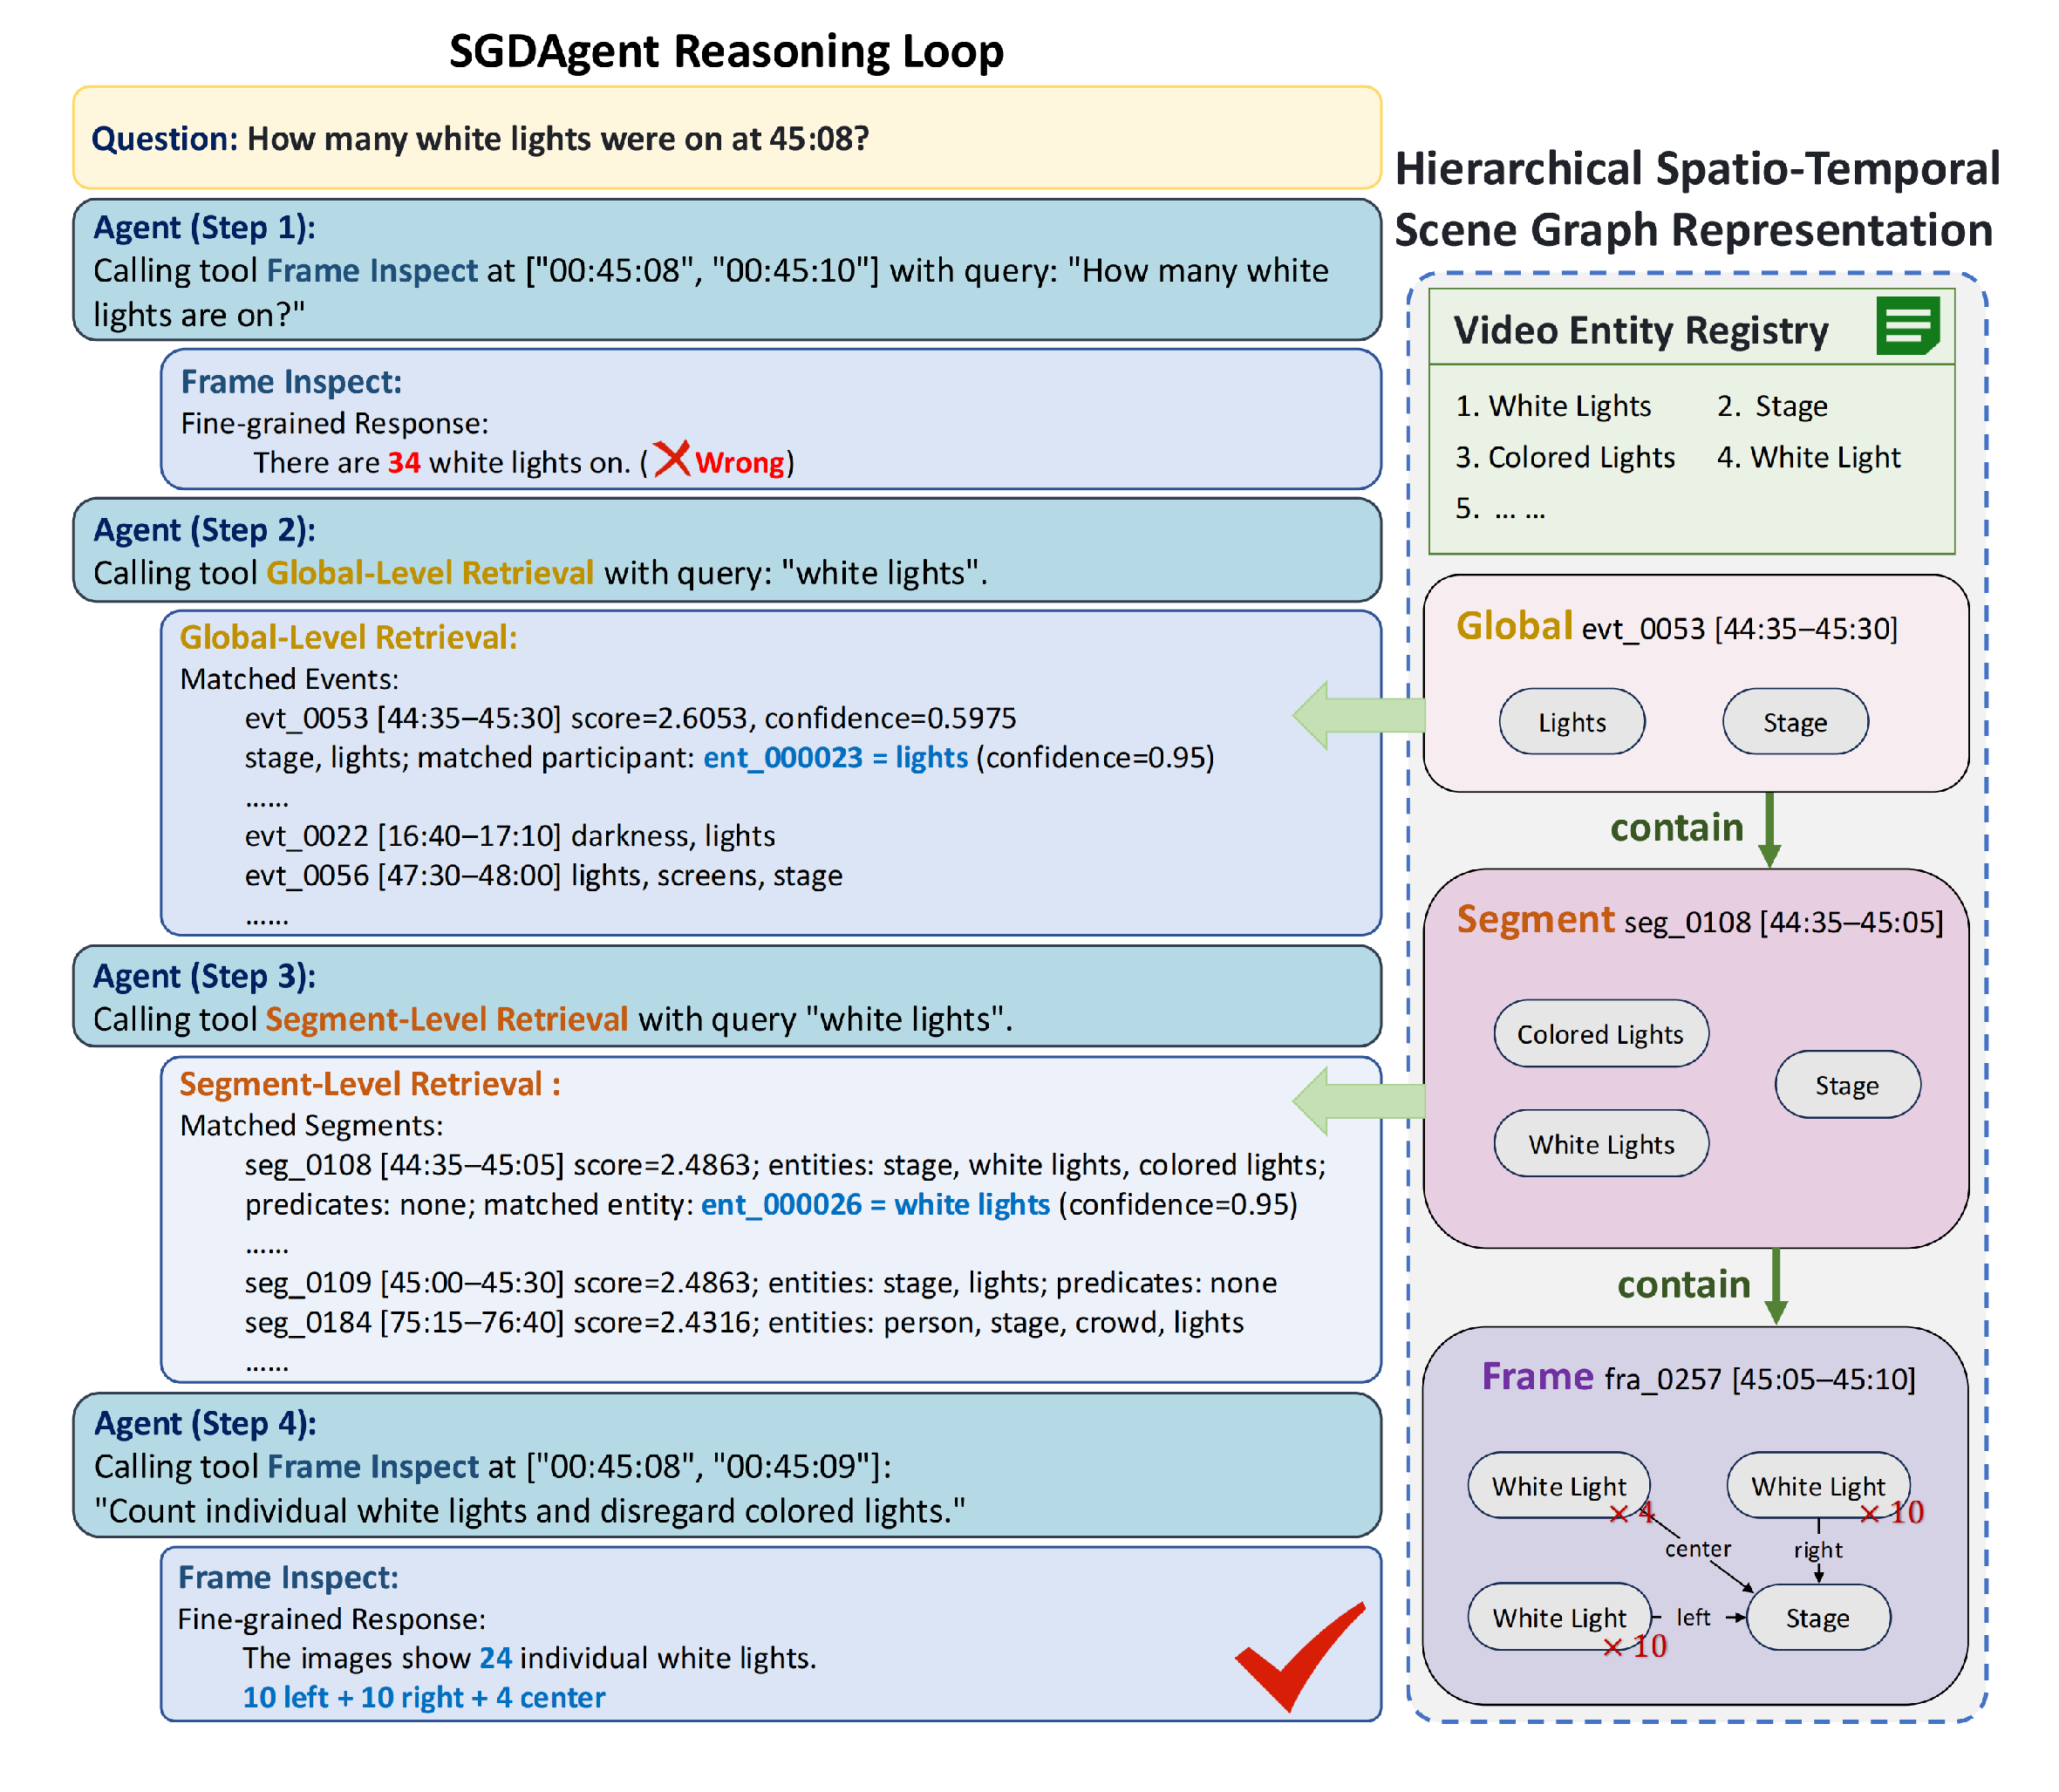
\includegraphics[width=\textwidth,height=0.88\textheight,keepaspectratio]{figures/Case_a1.pdf}
    \Description{A full-page case-study figure showing SGDAgent's reasoning trajectory for LVBench question 2256, including multi-step tool calls and the hierarchical scene graph evidence used to recover the correct count of white lights.}
    \caption{Case study from LVBench\cite{lvbench}, (qid: \texttt{2256}). SGDAgent reasoning trajectory on an exact counting example: graph-guided retrieval repairs an initially incorrect local probe and guides targeted visual verification to the correct answer.}
    \label{fig:appendix-case-a1}
\end{figure}

\begin{figure}[p]
    \centering
    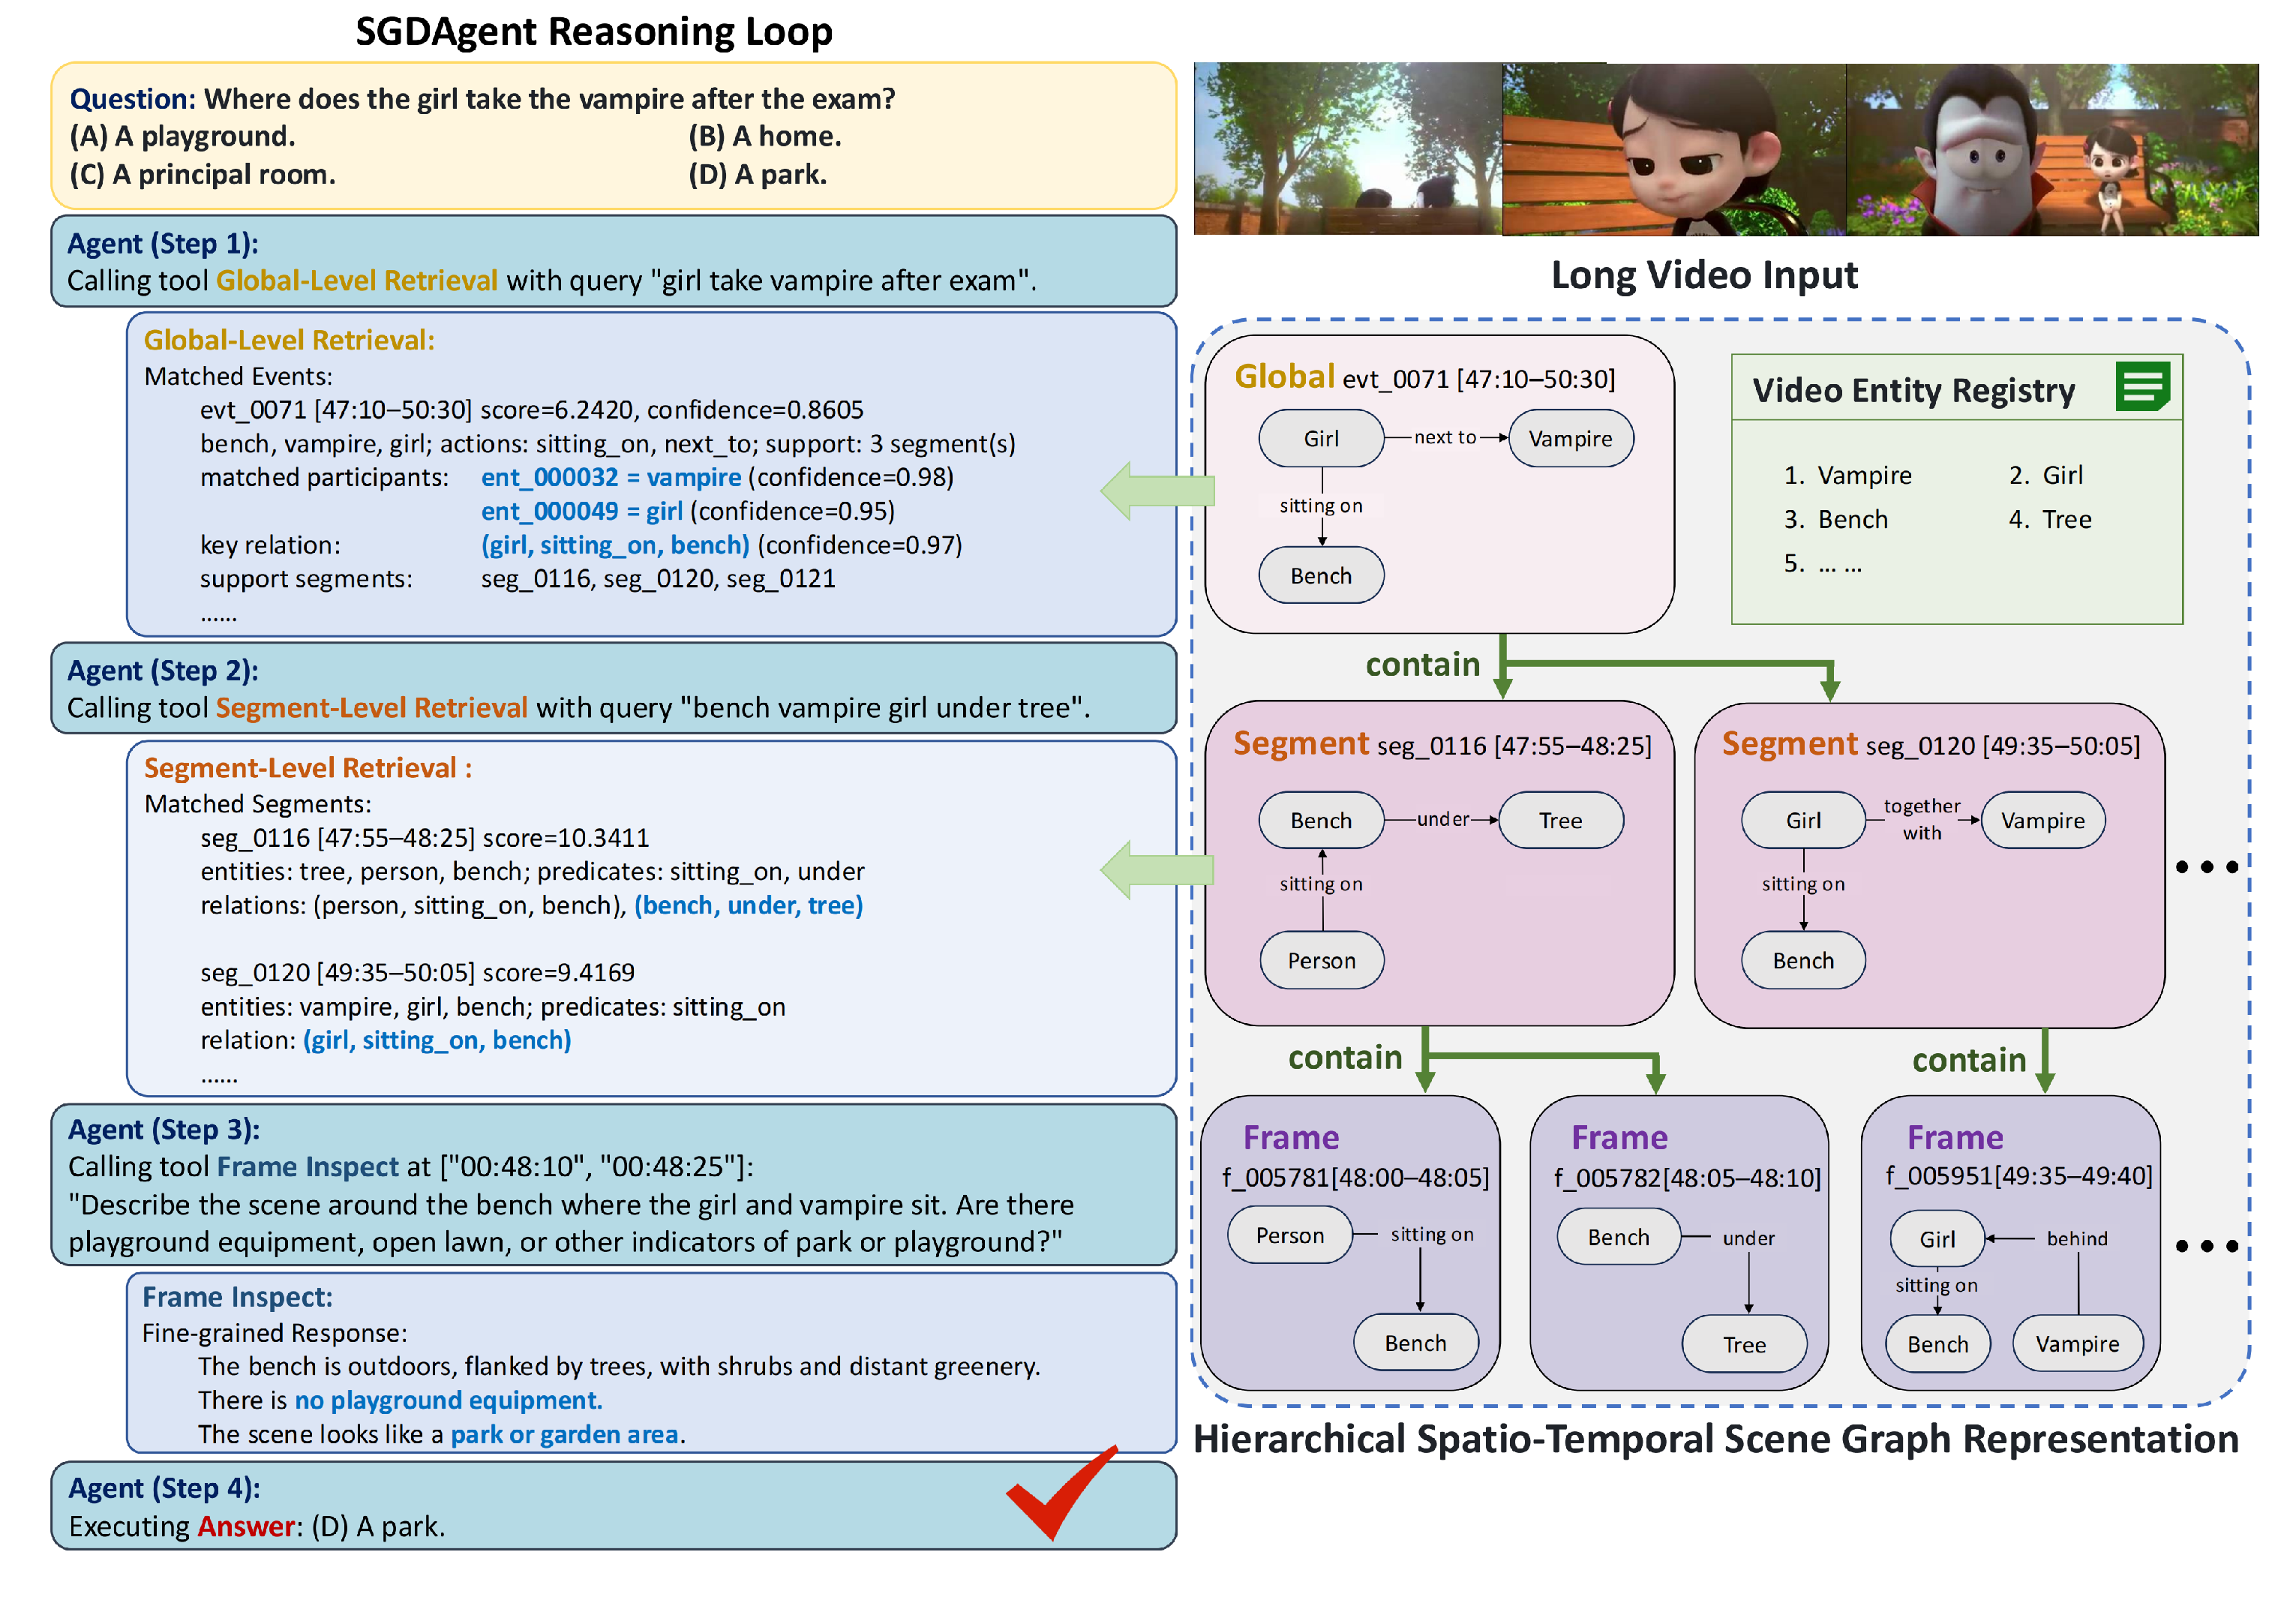
\includegraphics[width=\textwidth,height=0.88\textheight,keepaspectratio]{figures/Case_a2.pdf}
    \Description{A full-page case-study figure showing SGDAgent's reasoning trajectory for LVBench question 412, where graph retrieval localizes a park scene through entity-relation structure before a final visual verification step answers the question.}
    \caption{Case study from LVBench\cite{lvbench}, (qid: \texttt{412}). SGDAgent reasoning trajectory on a location QA example: graph queries progressively localize the answer around stable entity-relation structure before a single visual verification step commits the final answer.}
    \label{fig:appendix-case-a2}
\end{figure}

\begin{figure}[p]
    \centering
    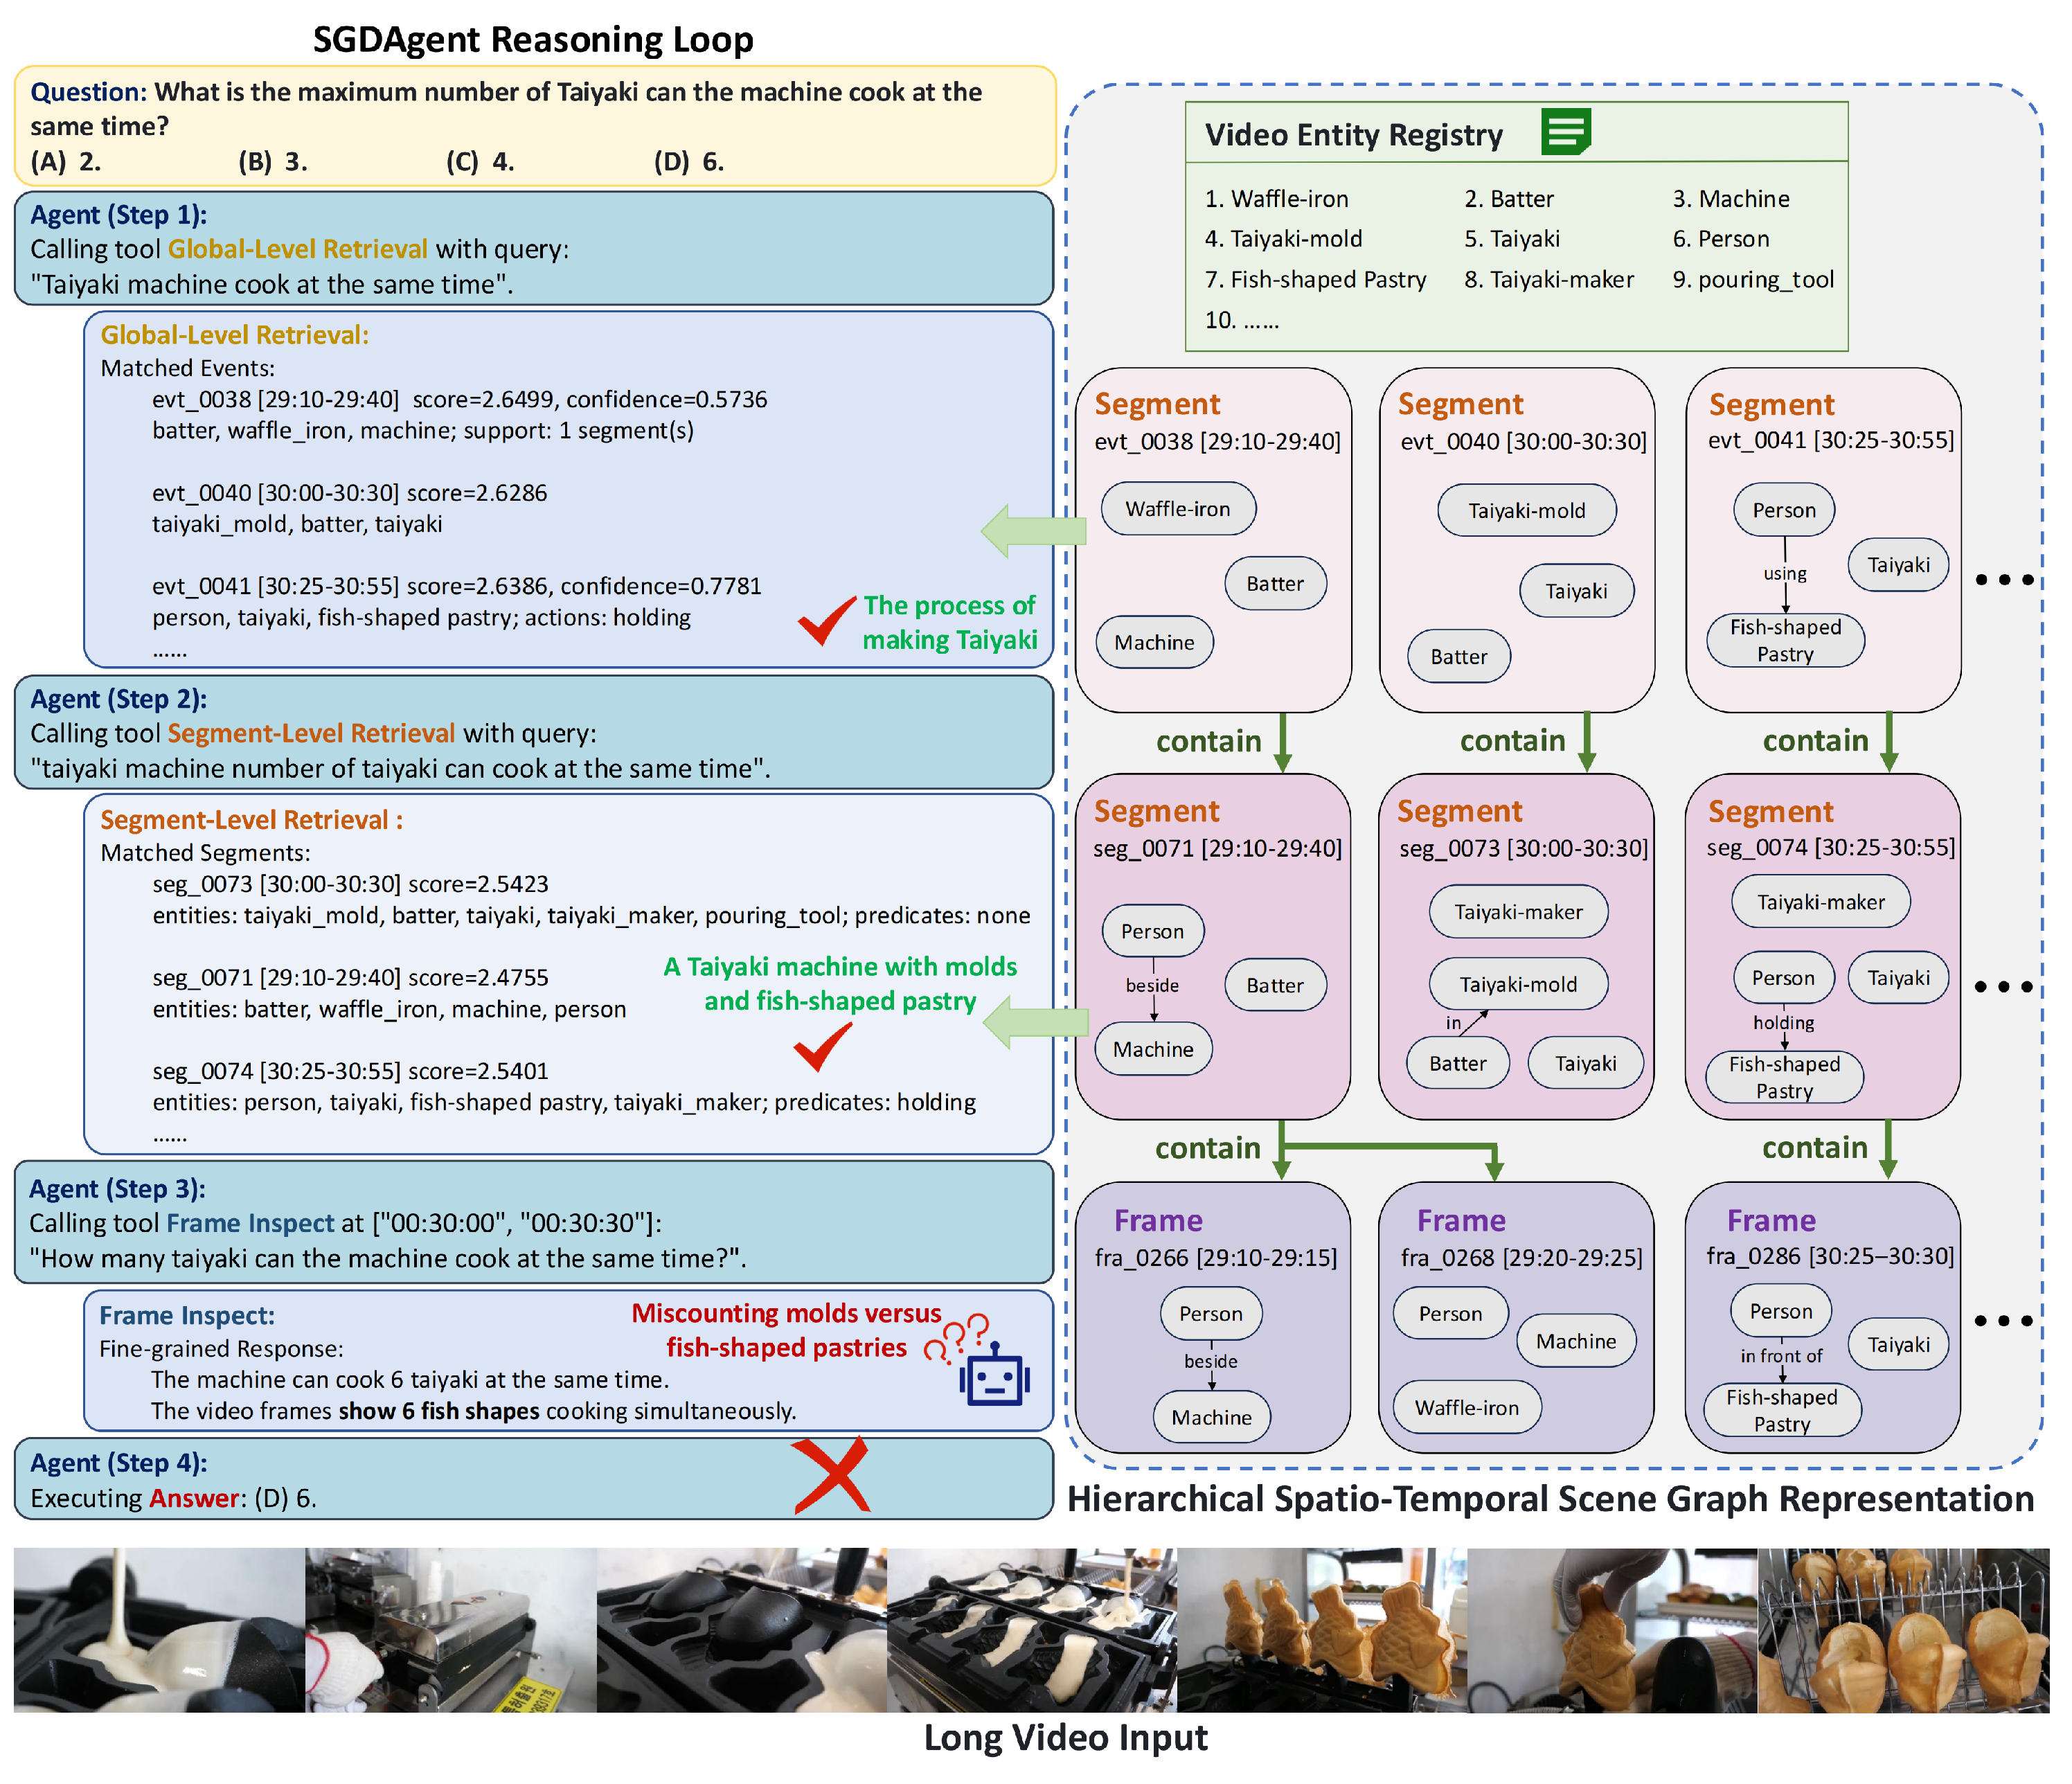
\includegraphics[width=\textwidth,height=0.88\textheight,keepaspectratio]{figures/Case_a3.pdf}
    \Description{A full-page failure-case figure showing SGDAgent's reasoning trajectory for LVBench question 3322, where the graph correctly localizes the Taiyaki cooking process but the final visual inspection overestimates the machine capacity.}
    \caption{Case study from LVBench\cite{lvbench}, (qid: \texttt{3322}). Failure case on numerical-state reasoning: the graph correctly localizes the cooking process, but the final visual inspection still overestimates the Taiyaki machine capacity.}
    \label{fig:appendix-case-a3}
\end{figure}

\end{document}
